\chapter{Code Transformations}\label{ch:two}

% Marginnote with a diagram here
\marginnote{
  An overview of the transformations\ldots
\begin{center}
  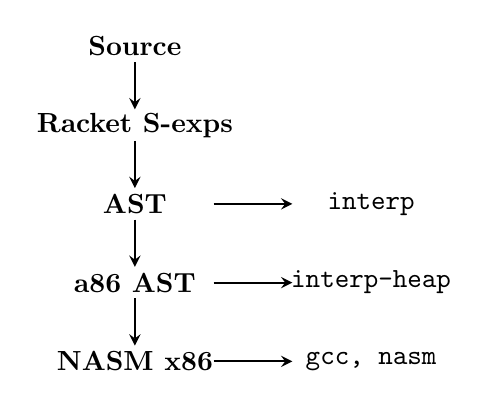
\begin{tikzpicture}
    \node at (0,0) {\textbf{Source}};
    \node at (0,-1) {\textbf{Racket S-exps}};

    \node at (0,-2) {\textbf{AST}};
    \node at (3,-2) {\texttt{interp}};

    \node at (0,-3) {\textbf{a86 AST}};
    \node at (3,-3) {\texttt{interp-heap}};

    \node at (0,-4) {\textbf{NASM x86}};
    \node at (3,-4) {\texttt{gcc, nasm}};

    \draw[thick, ->, >=stealth] (0,-0.2)--(0,-0.8);
    \draw[thick, ->, >=stealth] (0,-1.2)--(0,-1.8);
    \draw[thick, ->, >=stealth] (0,-2.2)--(0,-2.8);
    \draw[thick, ->, >=stealth] (0,-3.2)--(0,-3.8);

    \draw[thick, ->, >=stealth] (1,-2)--(2,-2);
    \draw[thick, ->, >=stealth] (1,-3)--(2,-3);
    \draw[thick, ->, >=stealth] (1,-4)--(2,-4);
\end{tikzpicture}
\end{center}
}

\newthought{From parsing to compilation}, Lonnrot Scheme code undergoes several
transformations before being either evaluated or simply transformed into NASM x86 code.
In this chapter, we explore the steps involved in each stage, the multiple
\textbf{intermediate representations} used, their characteristics and how these map
to the execution of a program.

% c.4
\section{Parsing}\label{sec:ch2_parsing}
The first stage of compilation is \textbf{parsing}, which in the case of Lonnrot
Scheme actually consists of two passes. \marginnote{Mostly for pedagogical purposes}
First, the source (a \textit{string}), is processed by a parser written in \texttt{megaparsack}.
By this point, from Chapter~\ref{ch:one}, we know that the result of this is a singular
\textit{s-expression}: a \texttt{begin} form. What now?

The next step in the process, found in \texttt{parse.rkt}, takes that form and uses pattern-matching
to recursively produce an AST representation. Possible nodes can be found in \texttt{ast.rkt}, but
the key takeaway is this: a program is a \texttt{Prog} Racket struct, whose fields are a list of
definitions (\texttt{Defs}) and a single expression.

\section{Desugaring}\label{sec:ch2_desugar}
Once we have our AST we could technically traverse it and evaluate the results, as
is the case of many interpreters. But we can also traverse it to pick out certain nodes, or even
\textit{transform it}. The latter is usually done in service of \textit{desugaring}, which simply
means that we can transform certain nodes of our tree into \textbf{core forms}.

This technique is used in Lonnrot in several ways: we can desugar \texttt{cond} into a sequence of
\texttt{if}s, we desugar \texttt{list} into a sequence of \texttt{cons} cells, but most importantly
we can desugar function definitions into a big \texttt{letrec}, which gives Lonnrot Scheme the
property of being able to have (1) mutually recursive functions and, generally (2) functions that
refer to functions defined later in the source.

% c.5
\section{The Environment}\label{sec:ch2_env}
In a typical Lisp interpreter, we can represent variable bindings through a structure
called an \textit{environment}, which is an \textbf{assoc-list}.\marginnote{An assoc-list, or
  association list, is simply a list of pairs, where the head (or car) of each element is a variable
  and the tail (or cdr, rest) of each element is the value associated to that variable}. In some ways
this may seem somewhat inefficient, but it plays to the \textbf{lexically scoped semantics} of the
language: it allows \textit{shadowing} since we extend the environment from the front. In other words,
by traversing the environment, you'll reach the latest definition of a given variable. A variable lookup,
naturally, consists of traversing the list, checking the \texttt{car} of each element.

The big insight behind this behavior is that, during compilation, we can represent stack memory as
a list. We do have to bear in mind a key difference: we don't know the value of variables during
compilation. How can we associate a value to a variable in this case? Well, \textbf{we don't} because
we \textbf{can't}; we lack information. What we do know is that we introduce bindings with
\texttt{let}, and we do have the structure of the code at compile-time. Therefore, we can
statically calculate the distance at which a variable's binding is supposed to be from the top
of the stack at runtime. In that sense, while a \texttt{lookup} in an interpreter simply traverses
an environment and returns a value, in compilation a \texttt{lookup} consists of traversing
the environment and returning \textit{an index}.
